\documentclass{beamer}

\usepackage[utf8]{inputenc}
\usepackage{hyperref}
%\usepackage{lmodern}
\usepackage[percent]{overpic}

\usepackage{listings}
\definecolor{mygreen}{RGB}{28,172,0} % color values Red, Green, Blue
\lstdefinestyle{limpo}{numbers=none}
\lstset{language=TeX,
    basicstyle=\small,
    commentstyle=\color{mygreen},%
    numbers=left,%
    numberstyle={\small \color{black}},% size of the numbers
    numbersep=9pt, % this defines how far the numbers are from the text
    emph=[1]{documentclass,usepackage,begin,end},emphstyle=[1]\color{blue}, %some words to emphasise
}

\newcommand{\tbs}{\textbackslash}

\author[Adriano Barbosa]{Adriano Barbosa\\
UFGD -- Universidade Federal da Grande Dourados\\
https://adrianobarbosa.xyz}
\title{Compress\~ao e reconstru\c{c}\~ao de imagens e a primeira foto de um buraco negro}
\subtitle[VI EMAAL]{VI Encontro de Matem\'atica do Agreste Alagoano}
\date{Outubro, 2019}

\beamertemplatenavigationsymbolsempty
\setbeamertemplate{caption}{\raggedright\insertcaption\par}
%\usetheme{Warsaw}
%\setbeamercolor{normal text}{fg=white,bg=black!90}
%\setbeamercolor{structure}{fg=white}
%\setbeamercolor{alerted text}{fg=red!85!black}
%\setbeamercolor{item projected}{use=item,fg=black,bg=item.fg!35}
%\setbeamercolor*{palette primary}{use=structure,fg=structure.fg}
%\setbeamercolor*{palette secondary}{use=structure,fg=structure.fg!95!black}
%\setbeamercolor*{palette tertiary}{use=structure,fg=structure.fg!90!black}
%\setbeamercolor*{palette quaternary}{use=structure,fg=structure.fg!95!black,bg=black!80}
%\setbeamercolor*{framesubtitle}{fg=white}
%\setbeamercolor*{block title}{parent=structure,bg=black!60}
%\setbeamercolor*{block body}{fg=black,bg=black!10}
%\setbeamercolor*{block title alerted}{parent=alerted text,bg=black!15}
%\setbeamercolor*{block title example}{parent=example text,bg=black!15}

\begin{document}

\begin{frame}
	\maketitle
\end{frame}

\begin{frame}{A primeira foto de um buraco negro}
    \begin{figure}
        \centering
        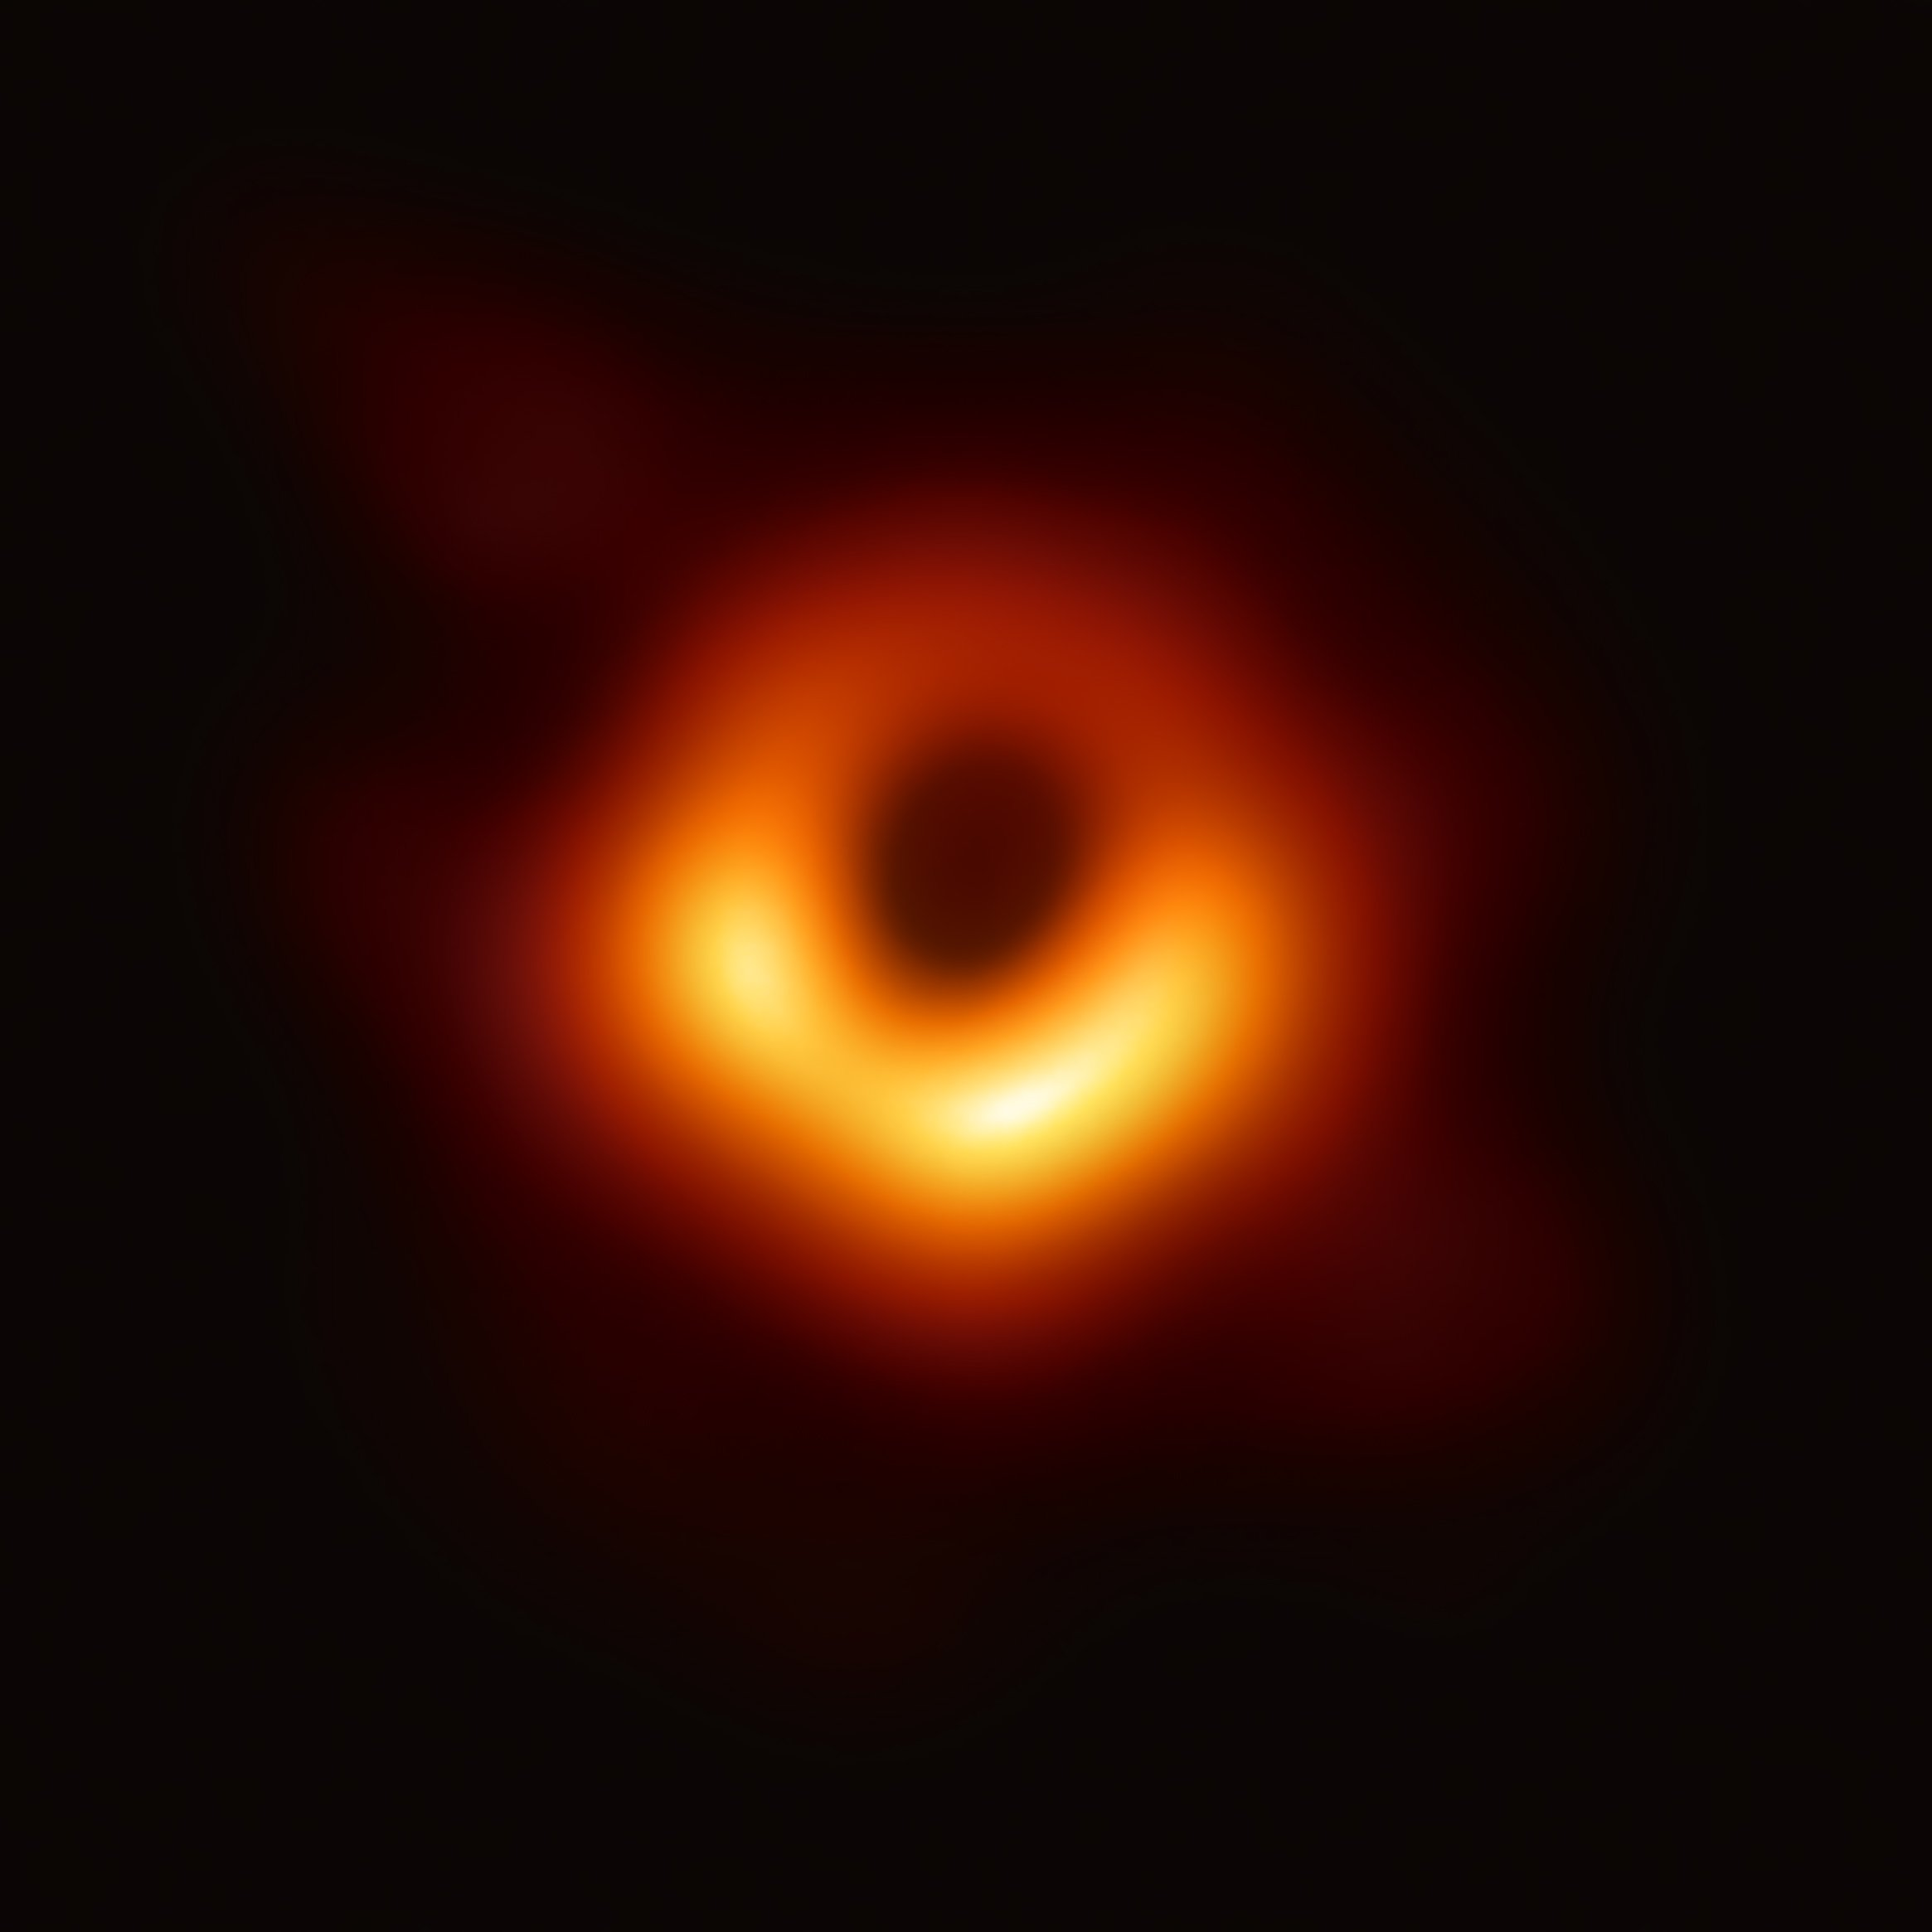
\includegraphics[width=0.6\textwidth]{figs/buraco-negro.jpg}
        \caption{Buraco negro da gal\'axia M87. Event Horizon Telescope, 2012 -- 2019}
    \end{figure}
\end{frame}

\begin{frame}{Katie Bouman}
    \begin{center}
        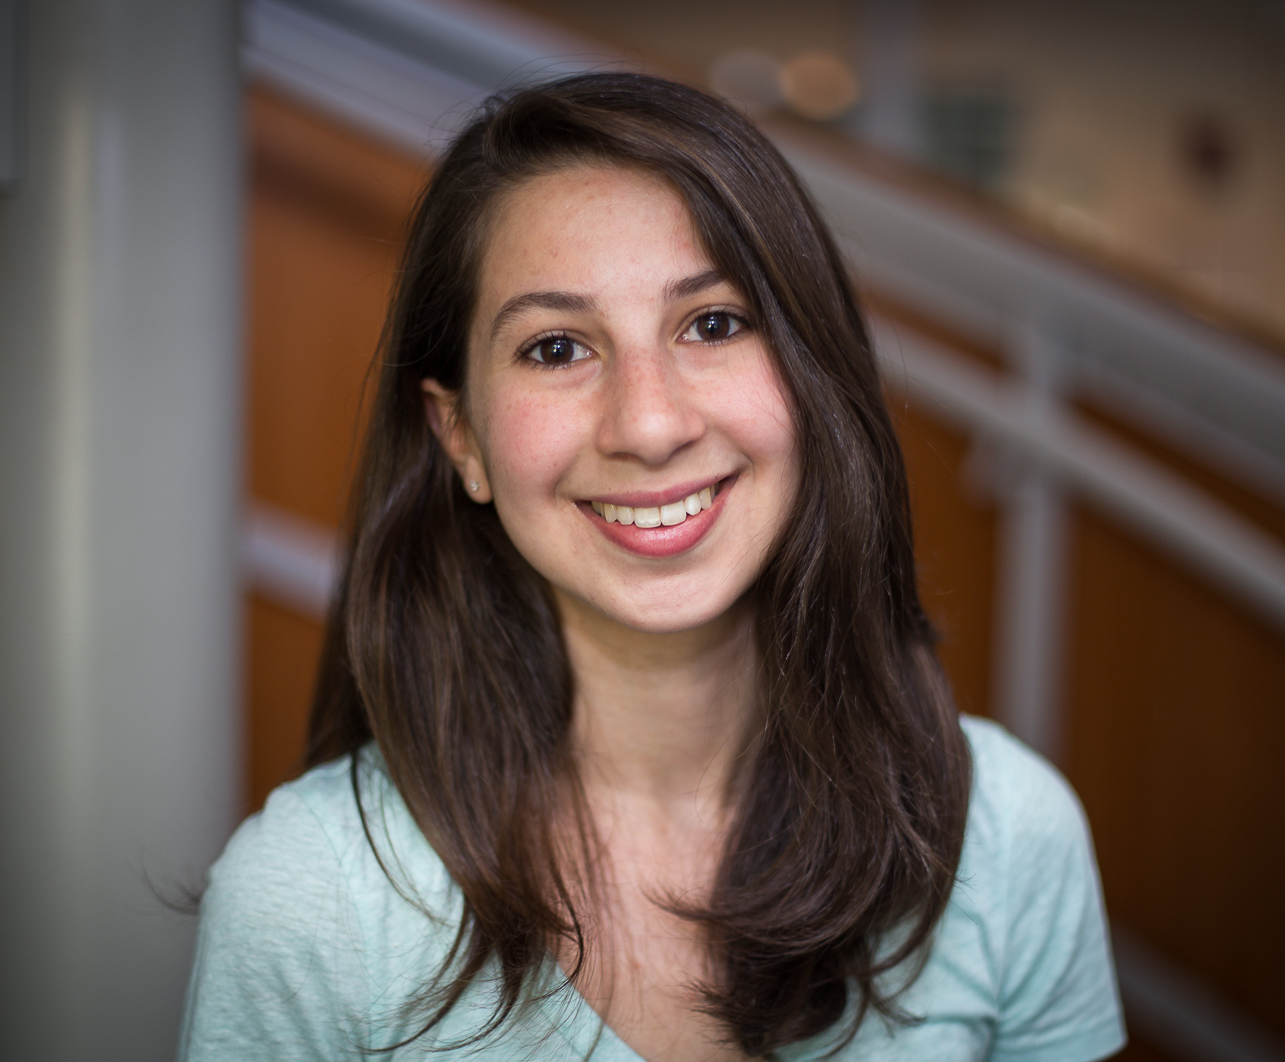
\includegraphics[height=4cm]{figs/katie.jpg}
    \end{center}
    \begin{itemize}
        \item Formada em engenharia el\'etrica \textit{cum laude}
        \item Pr\^emio Ernst Guillemin de melhor disserta\c{c}\~ao de mestrado
        \item Reconstruiu uma certa foto no doutorado
        \item Professora de ci\^encia da computa\c{c}\~ao no MIT
    \end{itemize}
\end{frame}

\begin{frame}{Katie Bouman}
    \begin{figure}
        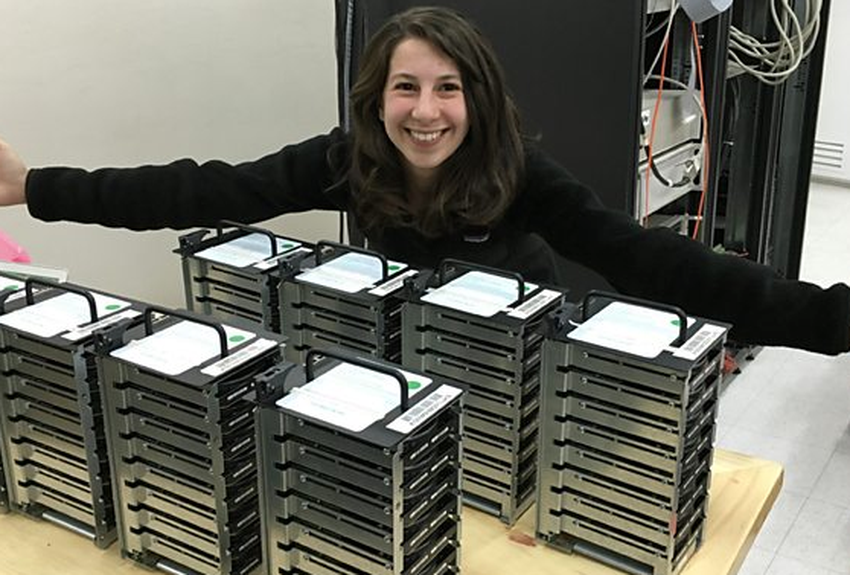
\includegraphics[width=0.48\textwidth]{figs/katie2.png}
        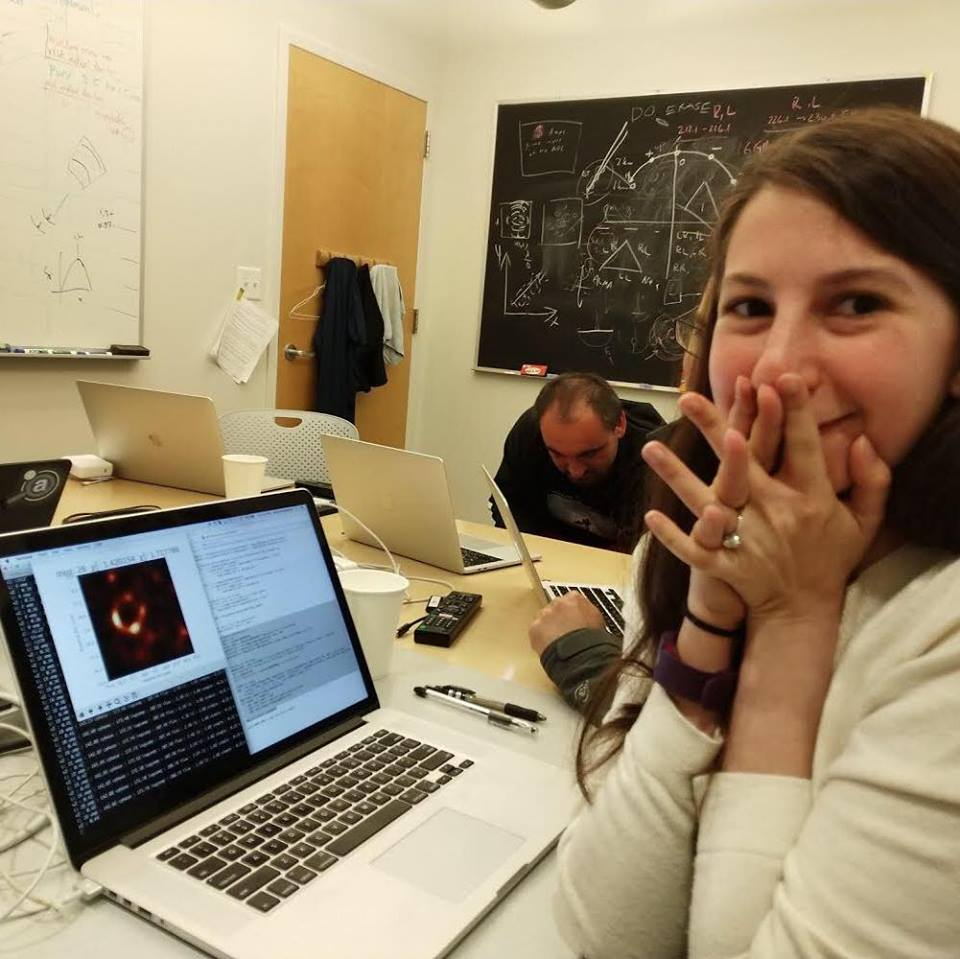
\includegraphics[width=0.48\textwidth]{figs/katie3.jpg}
    \end{figure}
\end{frame}

\begin{frame}{Como tirar a foto?}
    \[\text{tamanho do objeto} \approx \displaystyle\frac{\text{comprimento de
    onda}}{\text{tamanho do telesc\'opio}}\]
    \begin{center}
        Equivalente a fotografar uma laranja\footnote{Em cada pixel da imagem
        mais a direita cabem 1,5 milh\~oes de laranjas.} na lua!
    \end{center}
    \begin{figure}
        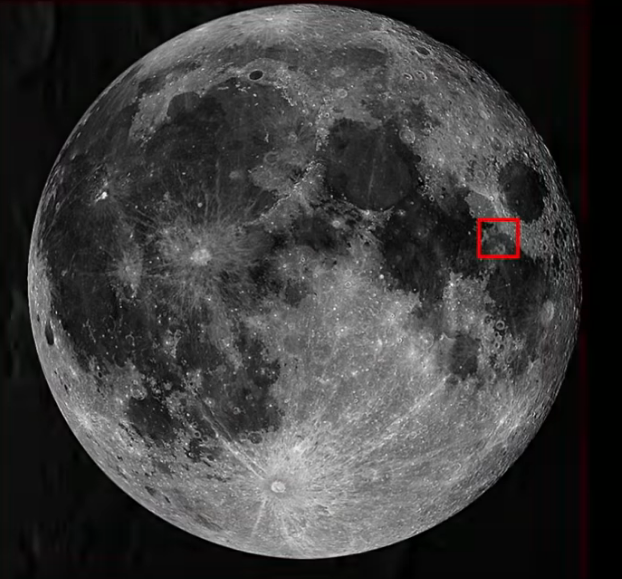
\includegraphics[width=0.27\textwidth]{figs/lua1.png}
        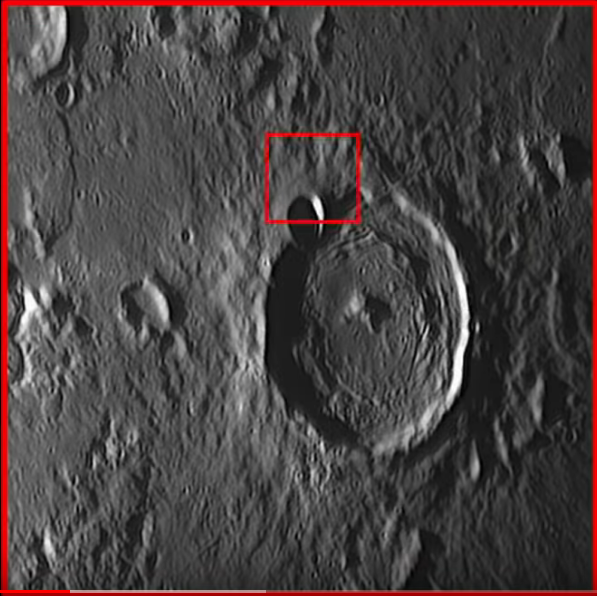
\includegraphics[width=0.25\textwidth]{figs/lua2.png}
        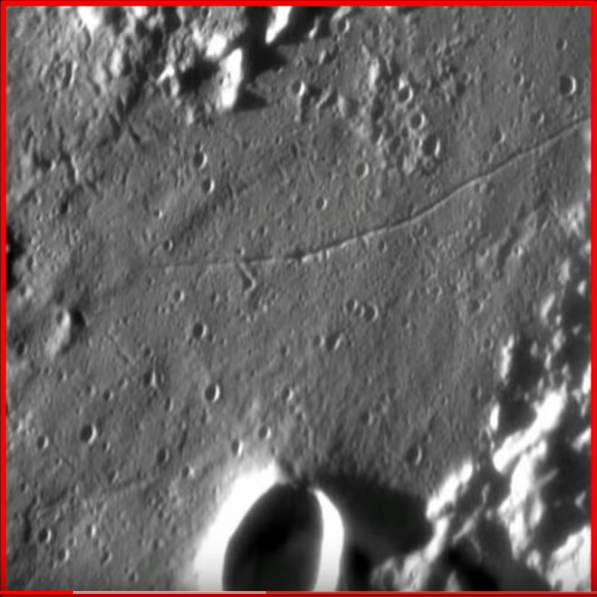
\includegraphics[width=0.25\textwidth]{figs/lua3.png}
        \caption{Fonte: Telesc\'opio Yepun, Paranal Observatory, Chile}
    \end{figure}
\end{frame}

\begin{frame}{Como tirar a foto?}
    \[\text{tamanho do objeto} \approx \displaystyle\frac{\text{comprimento de
    onda}}{\text{tamanho do telesc\'opio}}\]
    \begin{center}
        Precisamos de uma telesc\'opio do tamanho da Terra.
    \end{center}
    \pause{}
    \begin{figure}
        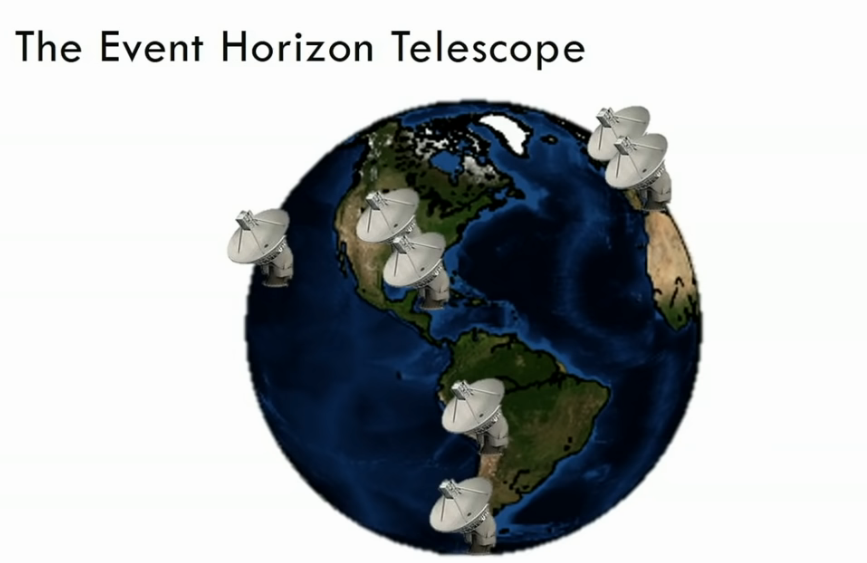
\includegraphics[scale=0.25]{figs/telescopios.png}
        \caption{Fonte: Katie Boulman, TED
        Talk (https://www.youtube.com/watch?v=BIvezCVcsYs)}
    \end{figure}
\end{frame}

\begin{frame}{O telesc\'opio}
    \begin{figure}
        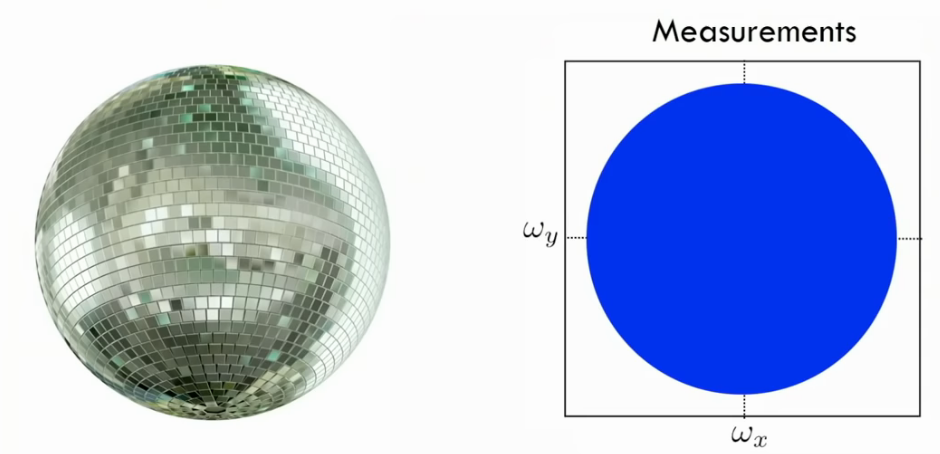
\includegraphics[scale=0.2]{figs/disco-ball1.png} \\
        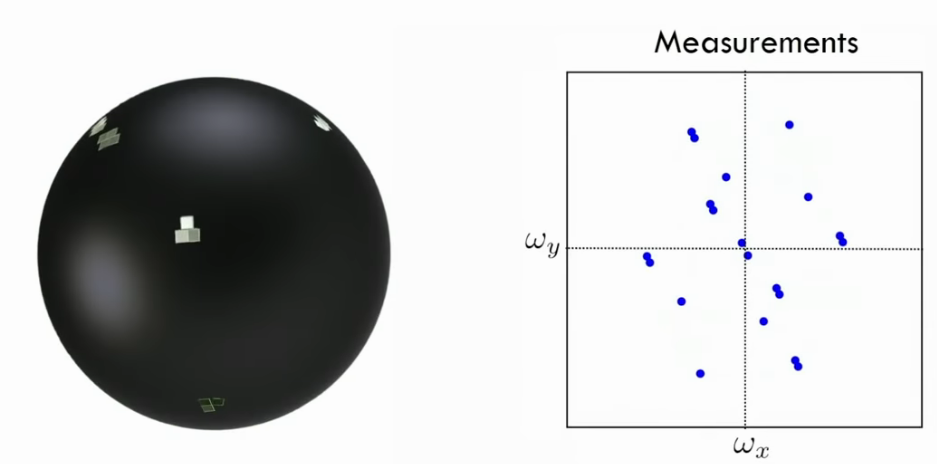
\includegraphics[scale=0.2]{figs/disco-ball2.png}
        \caption{Fonte: Katie Boulman, TED
        Talk (https://www.youtube.com/watch?v=BIvezCVcsYs)}
    \end{figure}
\end{frame}

\begin{frame}{O telesc\'opio}
    \begin{figure}
        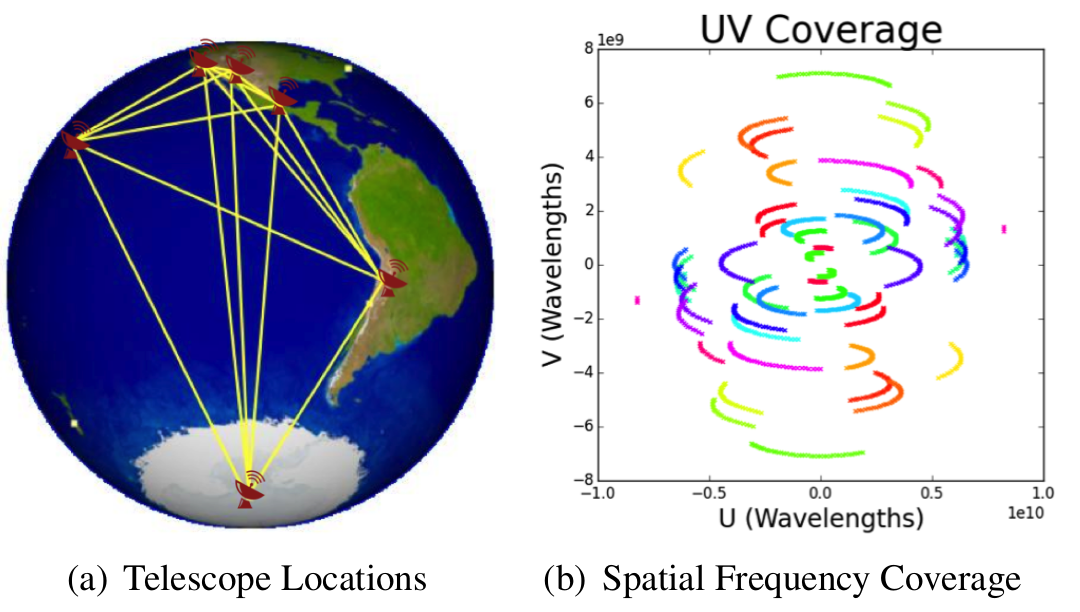
\includegraphics[scale=0.25]{figs/disco-ball3.png}
        \caption{Fonte: Bouman, K., et al. Computational Imaging for VLBI Image
        Reconstruction, CVPR 2016}
    \end{figure}
\end{frame}

\begin{frame}{Reconstru\c{c}\~ao}
    \begin{figure}
        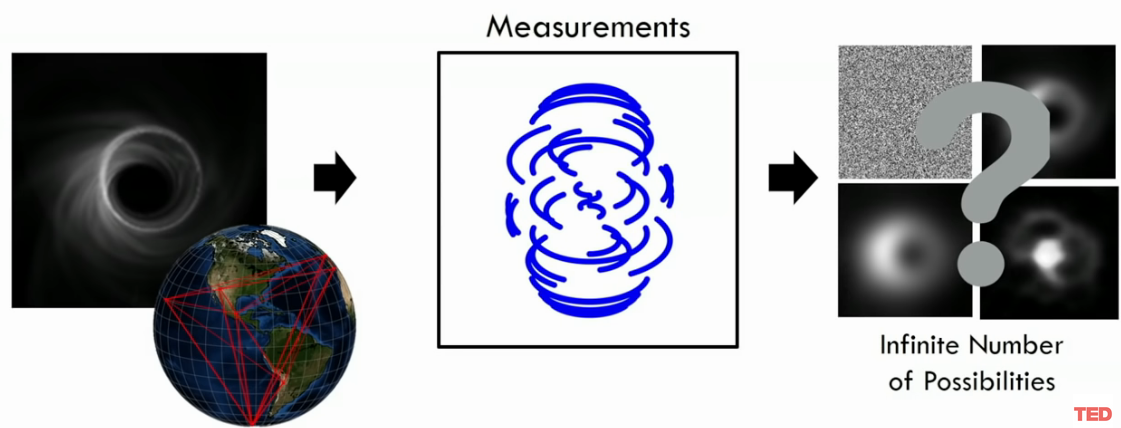
\includegraphics[scale=0.25]{figs/disco-ball4.png}
        \caption{Fonte: Katie Boulman, TED
        Talk (https://www.youtube.com/watch?v=BIvezCVcsYs)}
    \end{figure}
\end{frame}

\begin{frame}{Reconstru\c{c}\~ao}
    \begin{figure}
        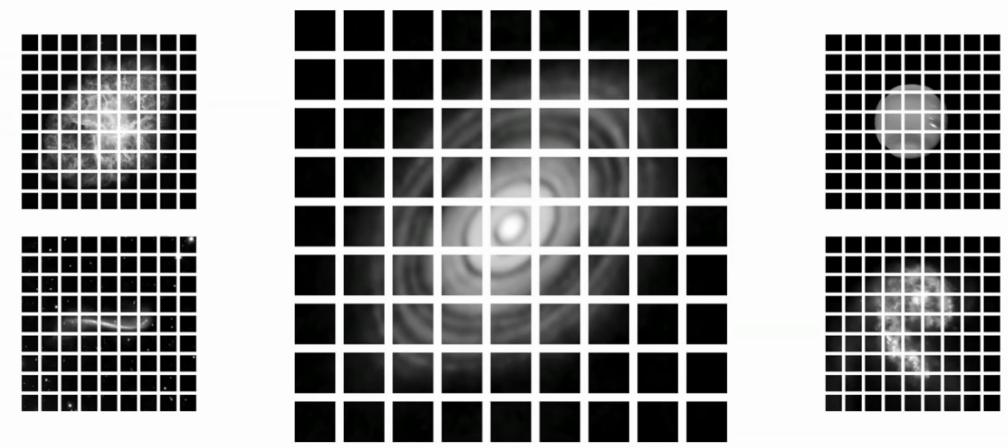
\includegraphics[width=\textwidth]{figs/reconstrucao1.png}
        \caption{Fonte: Katie Boulman, TED
        Talk (https://www.youtube.com/watch?v=BIvezCVcsYs)}
    \end{figure}
\end{frame}

\begin{frame}{Reconstru\c{c}\~ao}
    \begin{figure}
        
\includegraphics[width=0.3\textwidth]{figs/reconstrucao2.png}\hfill{}
        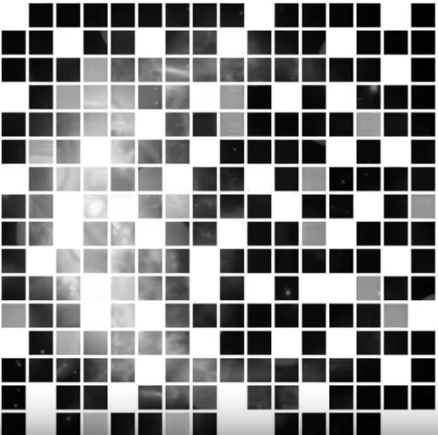
\includegraphics[width=0.3\textwidth]{figs/reconstrucao3.png}\hfill{}
        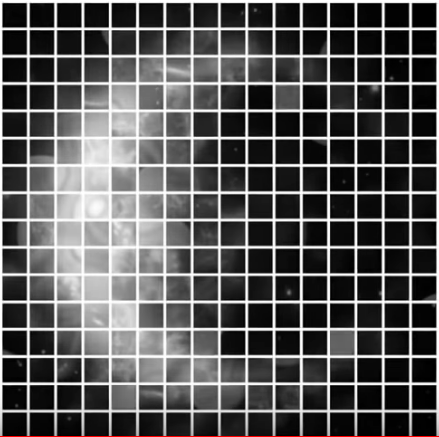
\includegraphics[width=0.3\textwidth]{figs/reconstrucao4.png}
        \caption{Fonte: Katie Boulman, TED
        Talk (https://www.youtube.com/watch?v=BIvezCVcsYs)}
    \end{figure}
\end{frame}

\begin{frame}{Reconstru\c{c}\~ao}
    \begin{figure}
        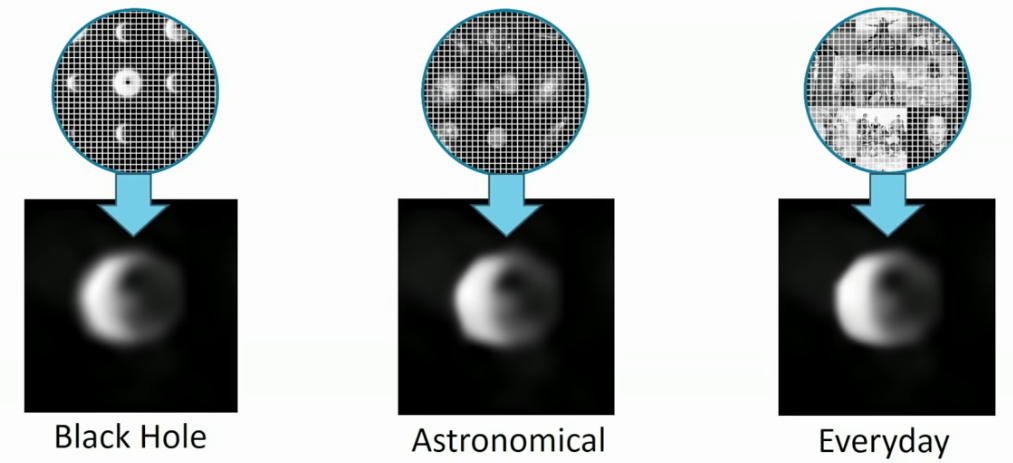
\includegraphics[width=\textwidth]{figs/reconstrucao5.png}\hfill{}
        \caption{Fonte: Katie Boulman, TED
        Talk (https://www.youtube.com/watch?v=BIvezCVcsYs)}
    \end{figure}
\end{frame}

%\begin{frame}{Modelagem de problemas}
%    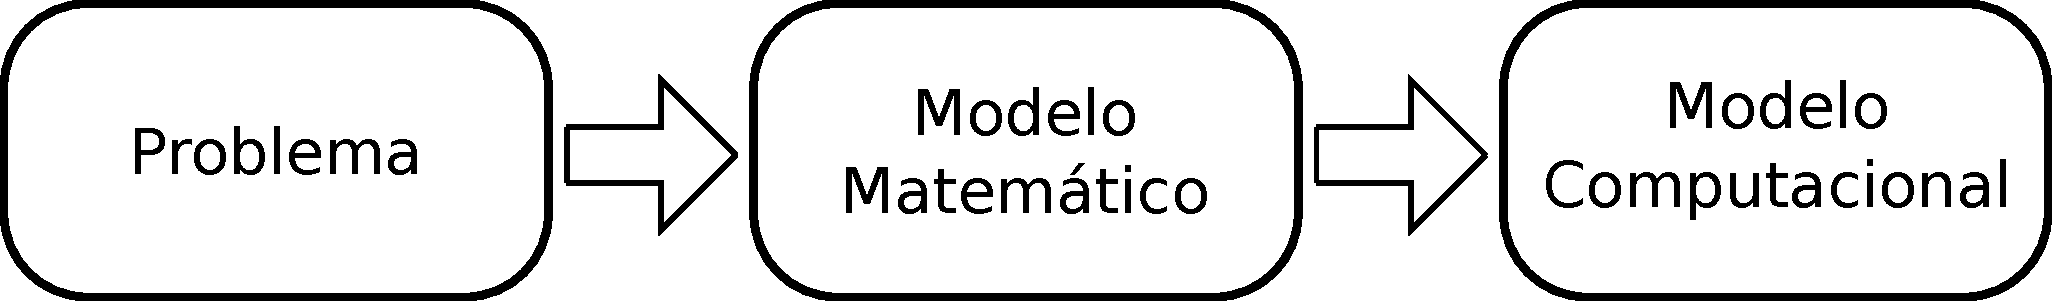
\includegraphics[width=\textwidth]{figs/paradigmas.pdf}
%\end{frame}

\begin{frame}{Nosso problema}
    \begin{center}
    Comprimir imagens no computador.
    \end{center}
\end{frame}

\begin{frame}{Como vemos uma imagem?}{Luz}
    \begin{figure}
        \centering
        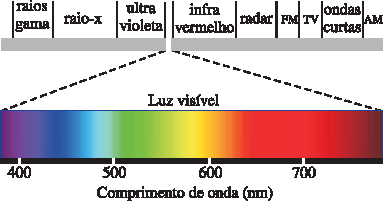
\includegraphics[scale=1.0]{figs/espectro-luz.pdf}
        \caption{Fonte: Gomes, J. e Velho, L., Fundamentos de Computa\c{c}\~ao
        Gr\'afica}
    \end{figure}
\end{frame}

\begin{frame}{Como vemos uma imagem?}{Olho}
    \begin{figure}
        \centering
        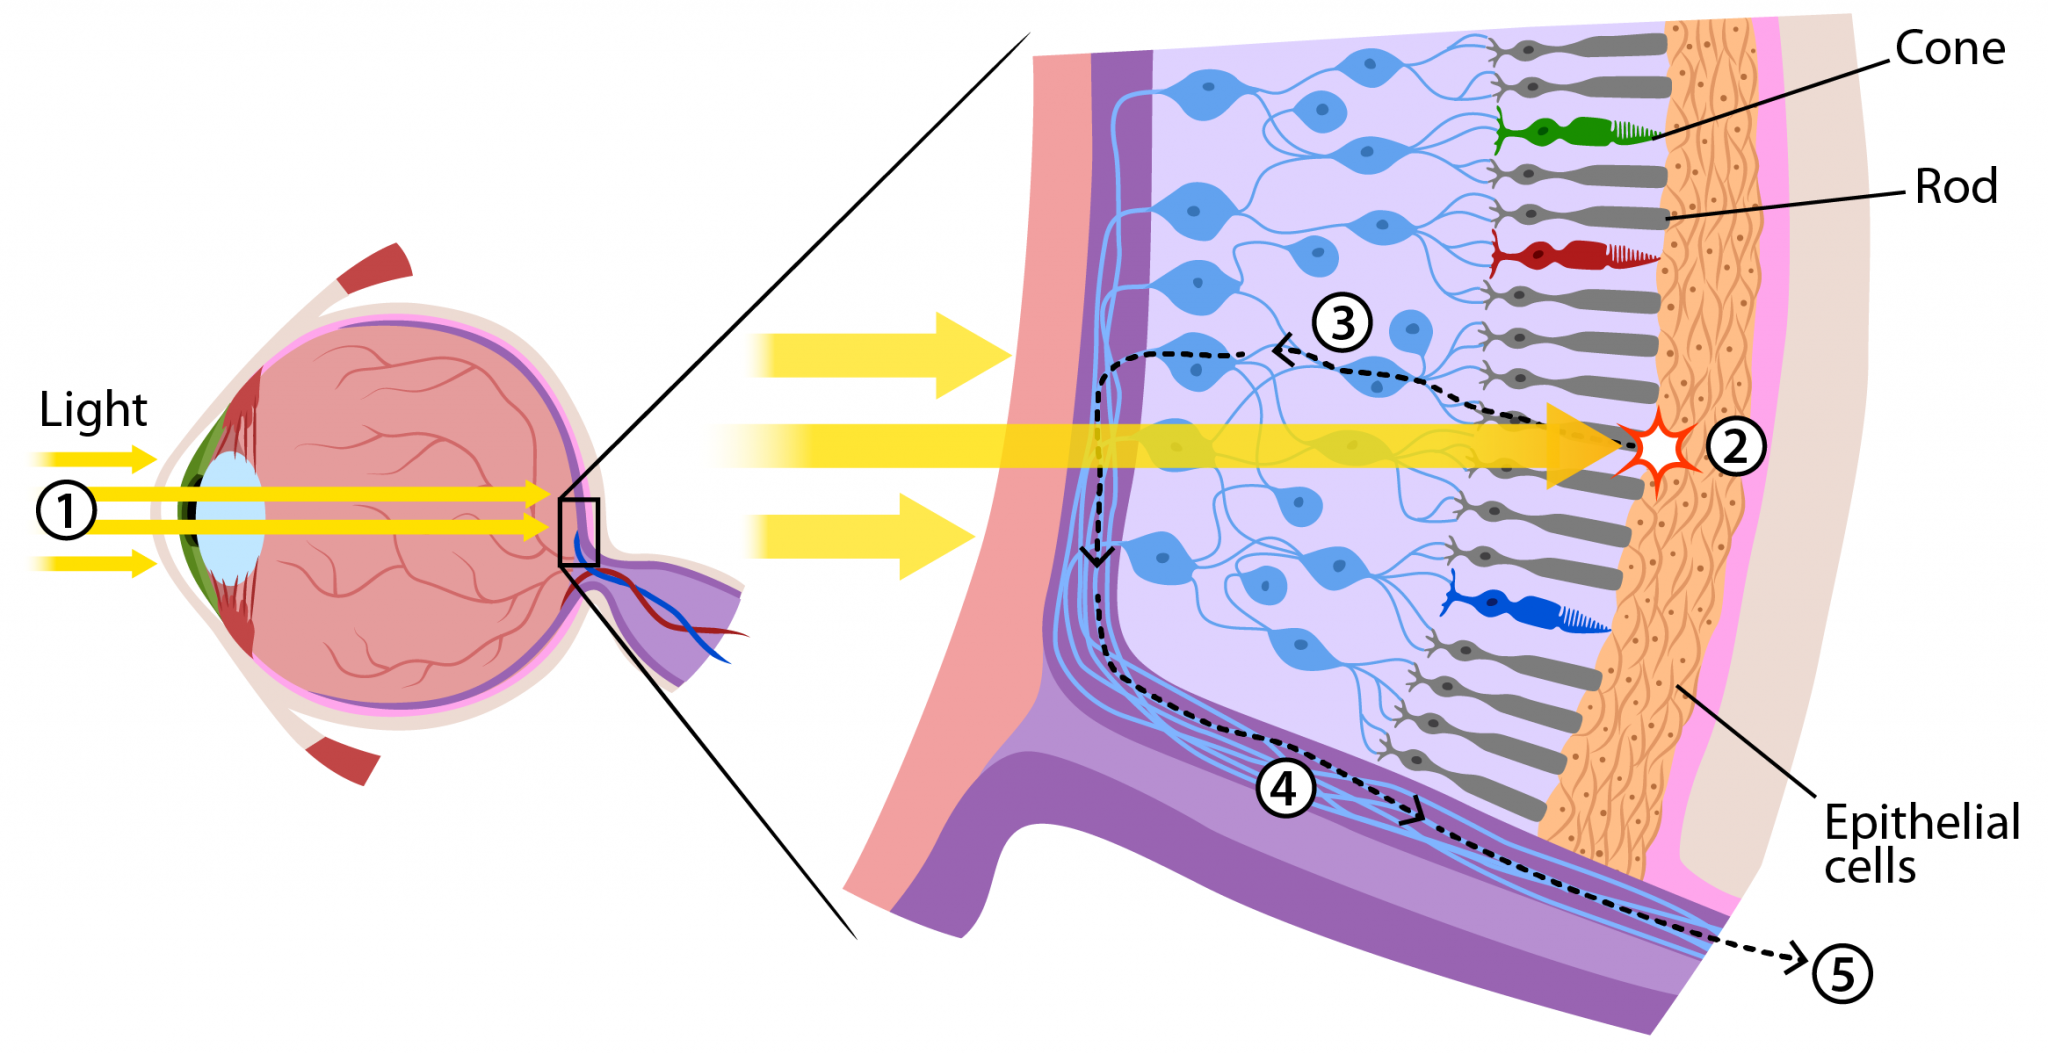
\includegraphics[width=\textwidth]{figs/rods-cones.png}
        \caption{Fonte: https://askabiologist.asu.edu/rods-and-cones}
    \end{figure}
\end{frame}

\begin{frame}{Como vemos uma imagem?}{Sistema {\color{red}R}{\color{green}G}{\color{blue}B}}
    \begin{figure}
        \centering
        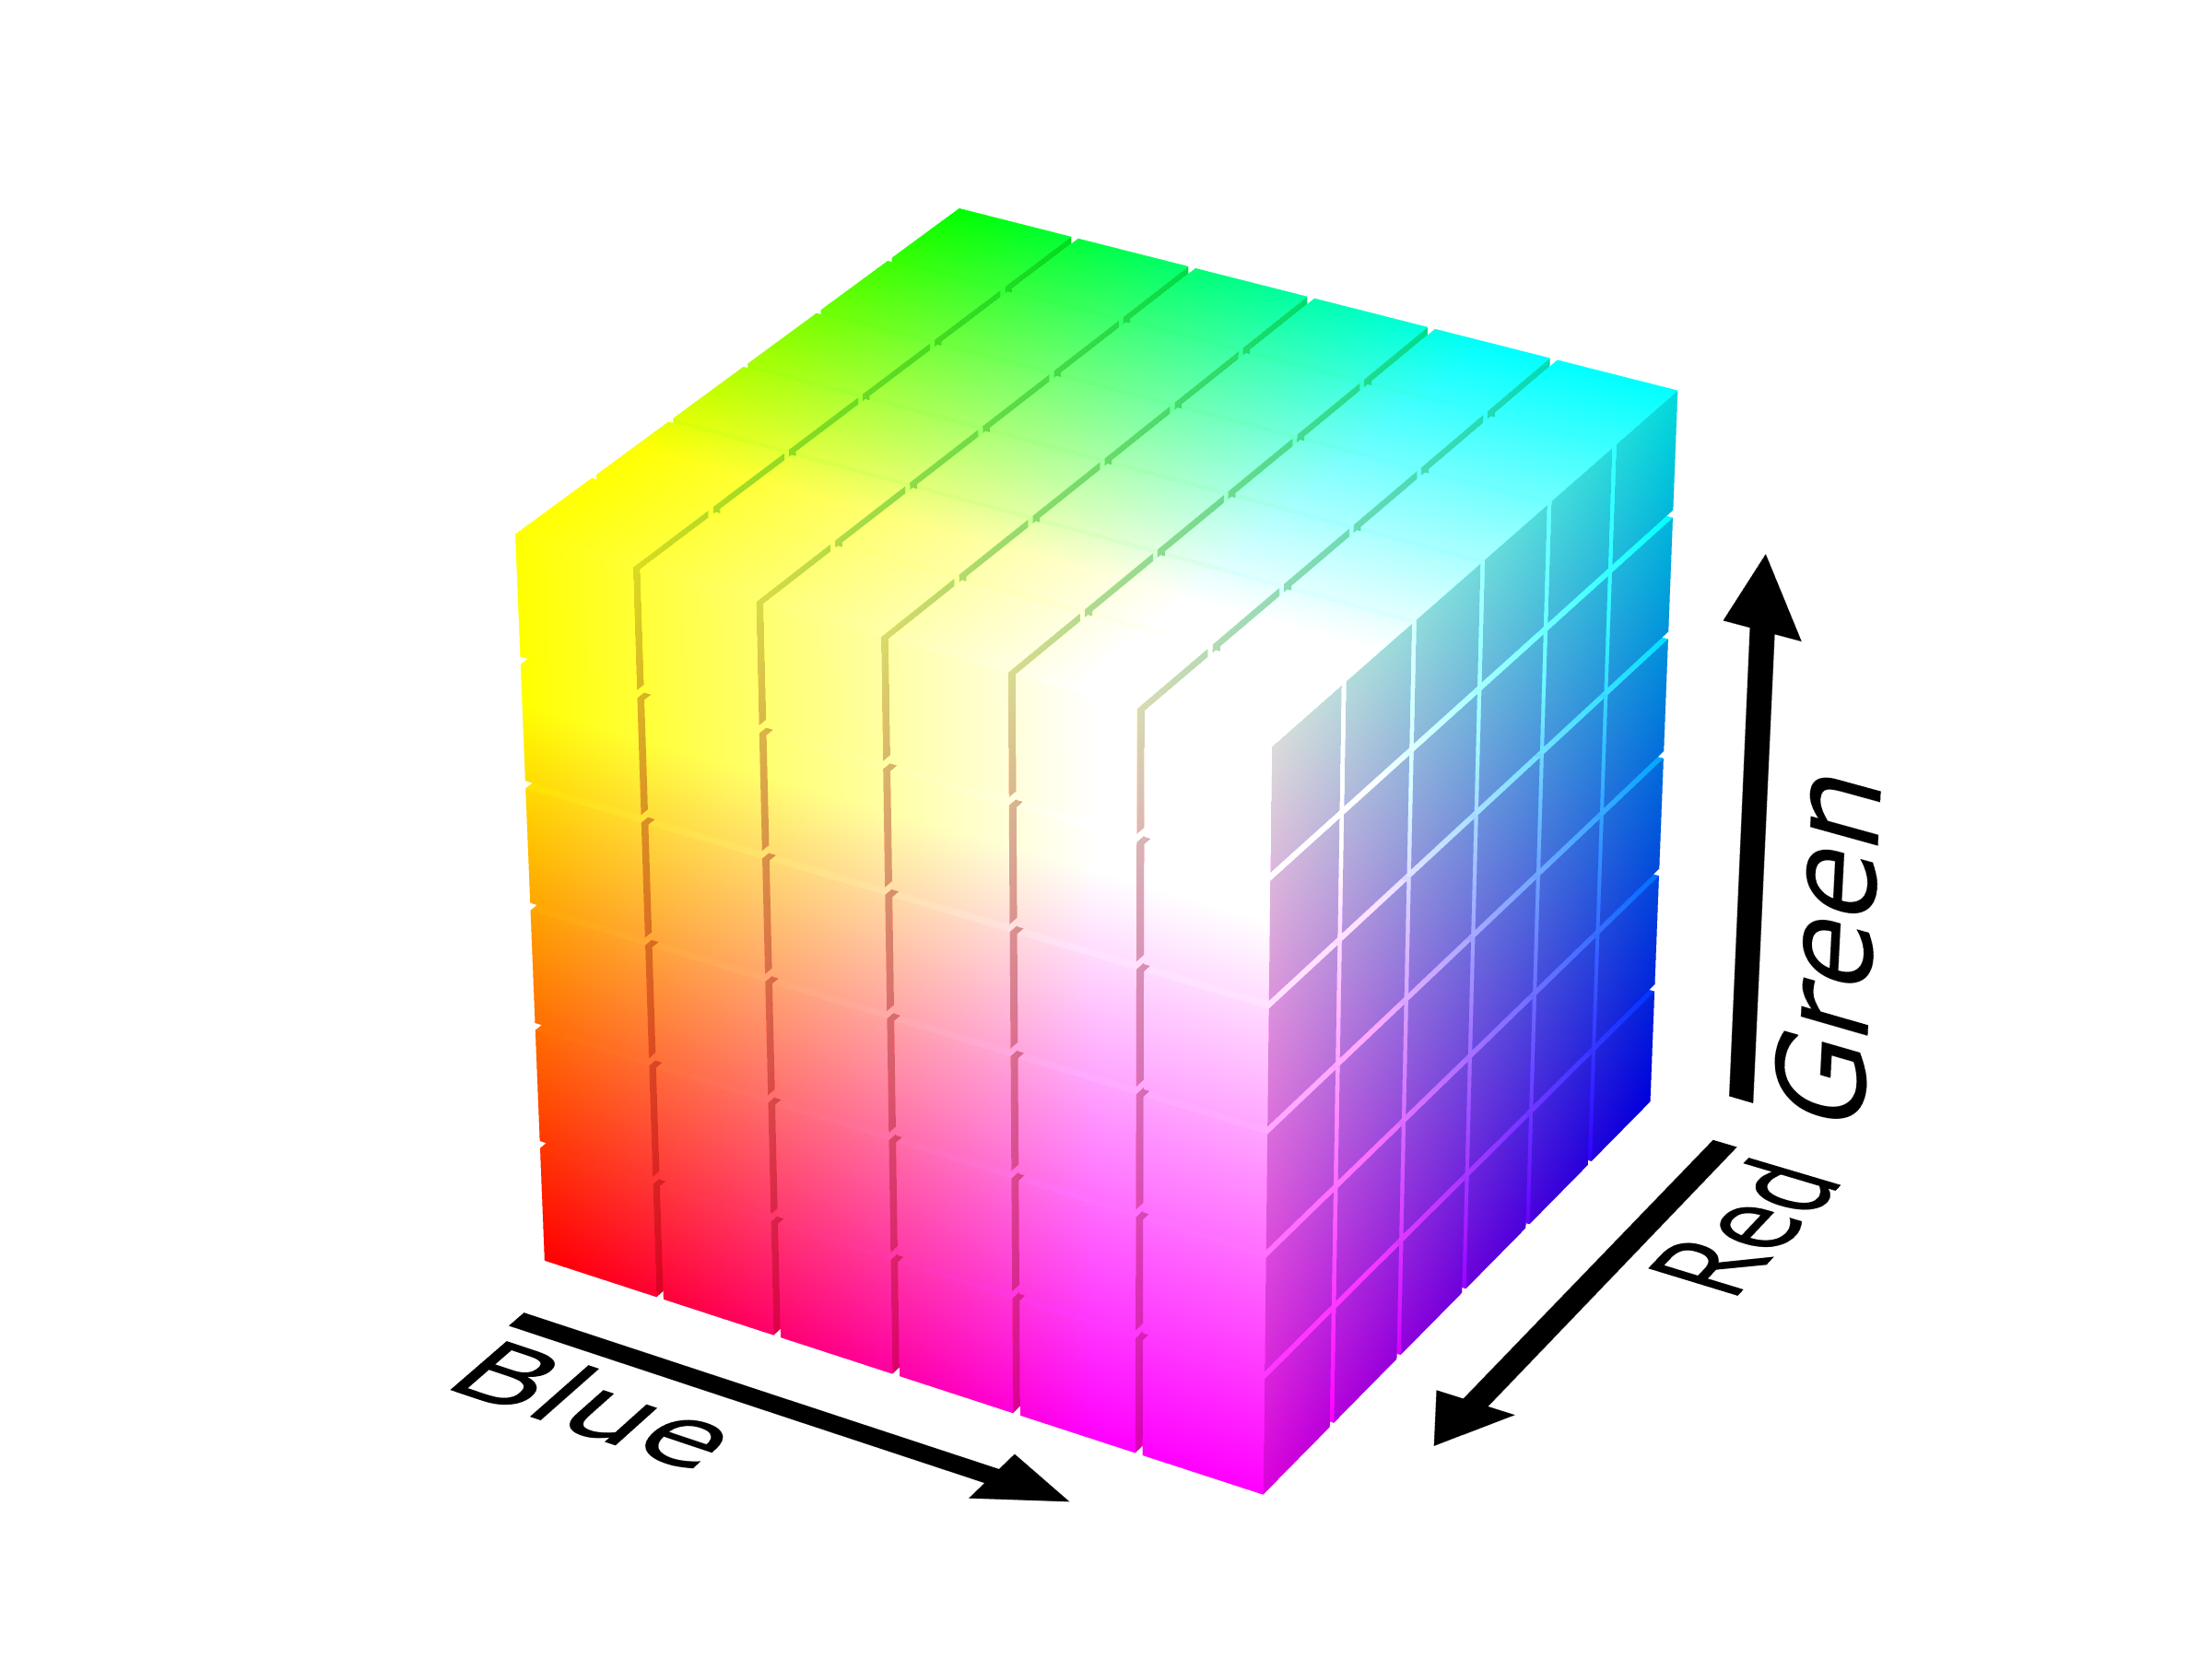
\includegraphics[width=0.8\textwidth]{figs/rgb-cube.png}
        \caption{Fonte: https://en.wikipedia.org/wiki/RGB\_color\_model}
    \end{figure}
\end{frame}

\begin{frame}{Como vemos uma imagem?}{Sistema {\color{red}R}{\color{green}G}{\color{blue}B}}
    \begin{figure}
        \centering
        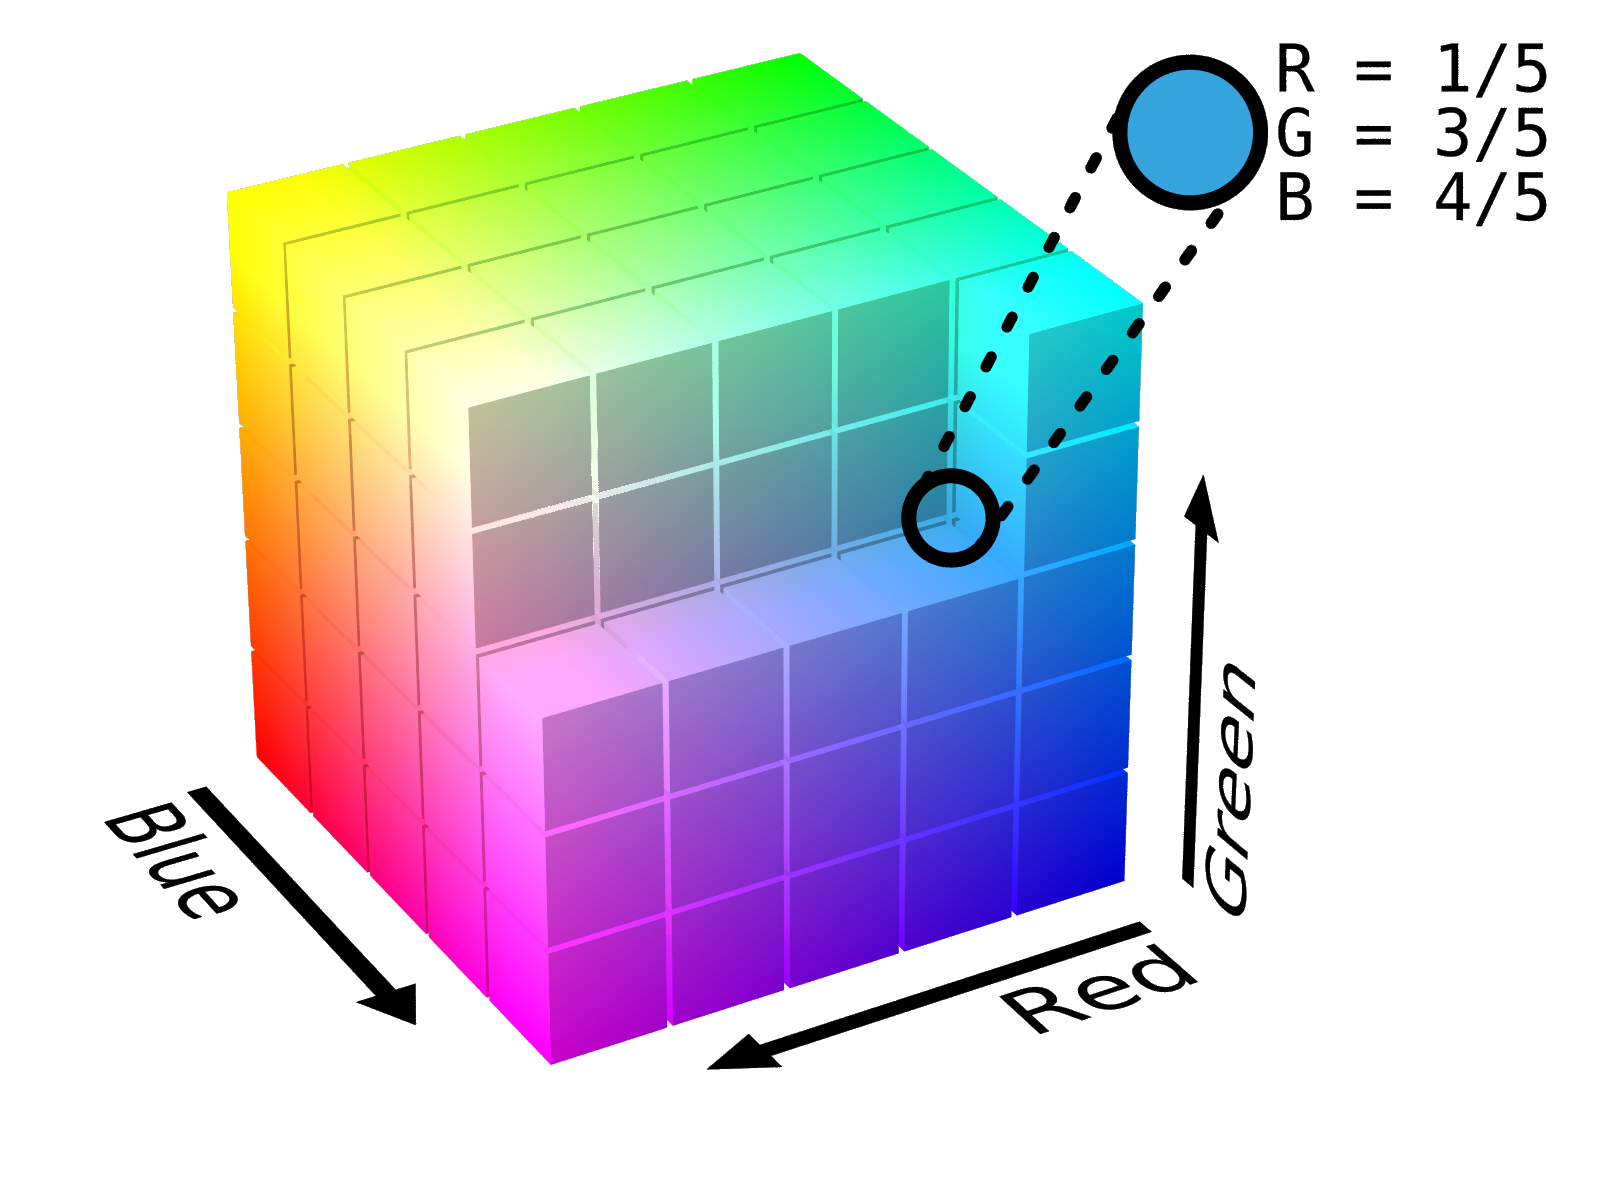
\includegraphics[width=0.8\textwidth]{figs/rgb-point.png}
        \caption{Fonte: https://en.wikipedia.org/wiki/RGB\_color\_space}
    \end{figure}
\end{frame}

\begin{frame}{Uma imagem no computador}
    \begin{figure}
        \centering   
        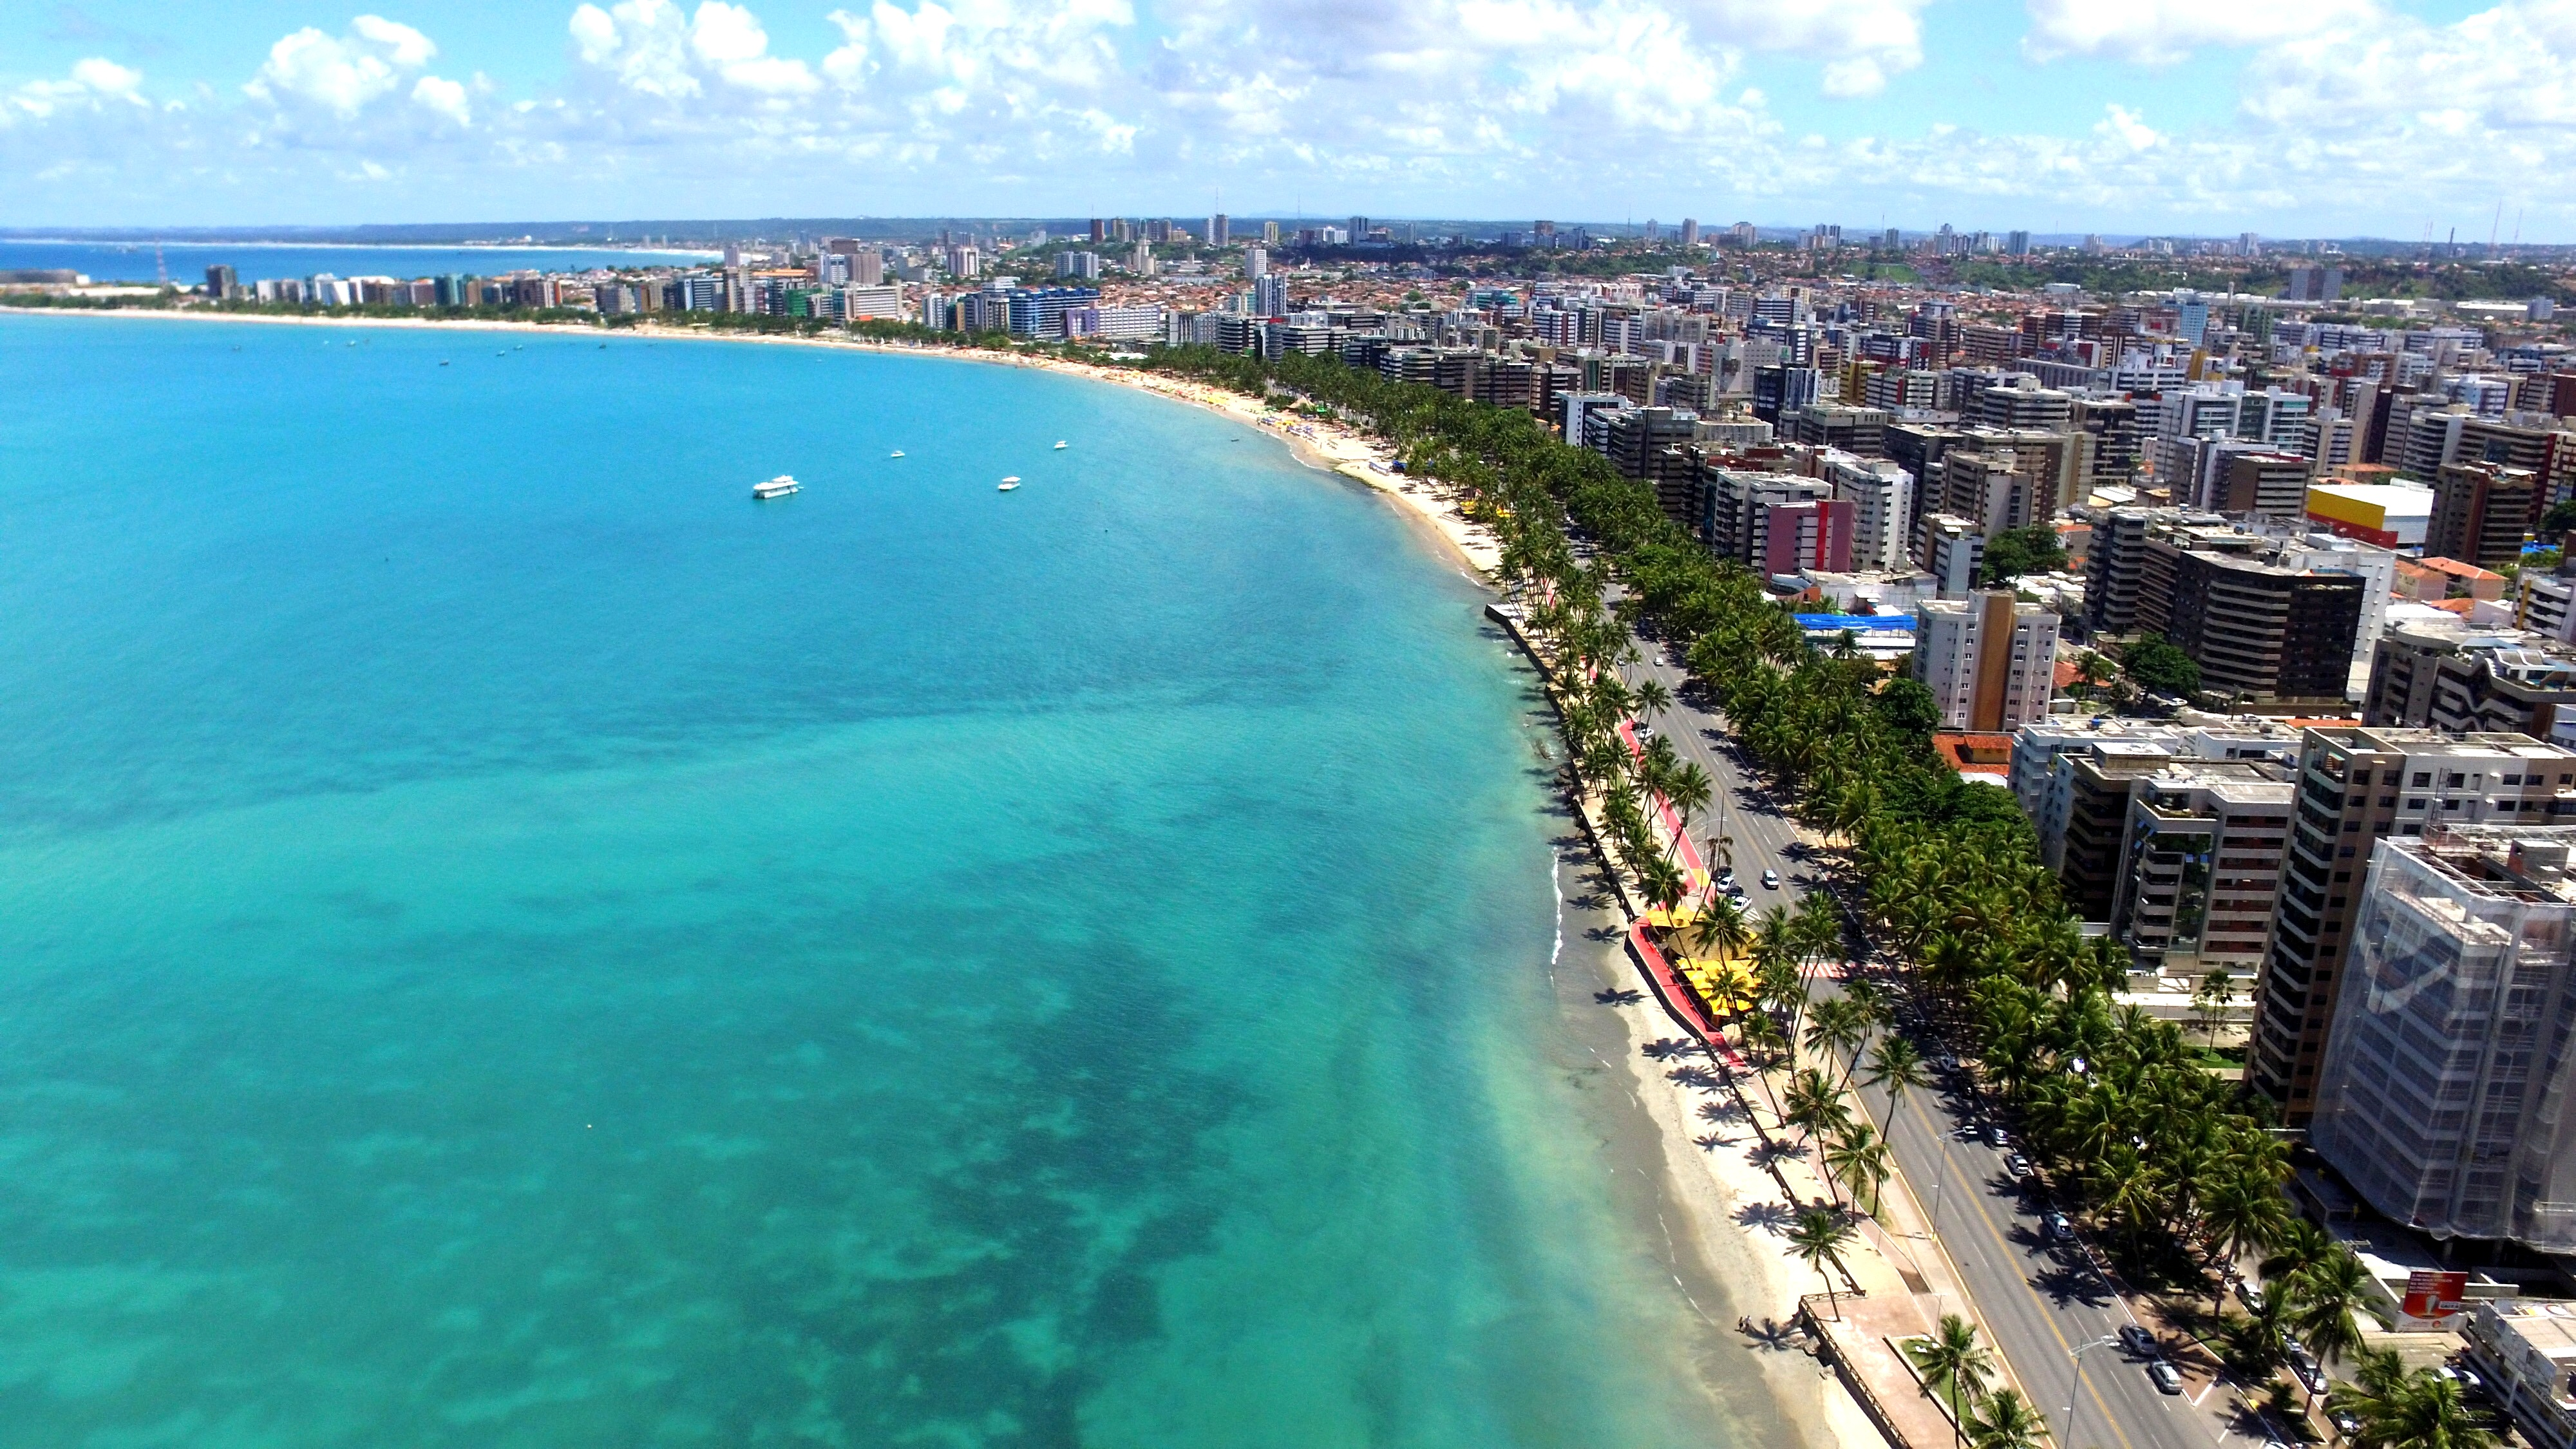
\includegraphics[width=\textwidth]{figs/maceio.jpg}
        \caption{Fonte: M\'arcio no Mundo}
    \end{figure}
\end{frame}

\begin{frame}{Uma imagem no computador}
    \begin{figure}
        \centering   
        \begin{overpic}[width=\textwidth]{figs/maceio.jpg}
            \put(3,3){
\includegraphics[width=0.5\textwidth]{figs/maceio-zoom1.png}}  
        \end{overpic}
        \caption{Fonte: M\'arcio no Mundo}
    \end{figure}
\end{frame}

\begin{frame}{Uma imagem no computador}{Matrizes}
    \begin{figure}
        \centering   
        
\includegraphics[scale=0.2]{figs/maceio-zoom2.png}
    \end{figure}
\end{frame}

\begin{frame}{Uma imagem no computador}{Matrizes}
    \begin{figure}
        \centering   
        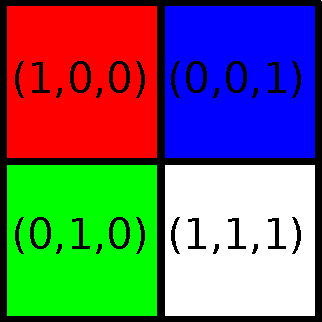
\includegraphics[width=0.5\textwidth]{figs/imagem-matriz.pdf}
    \end{figure}
\end{frame}

\begin{frame}{Uma imagem no computador}{Matrizes}
    \begin{figure}
        \centering   
        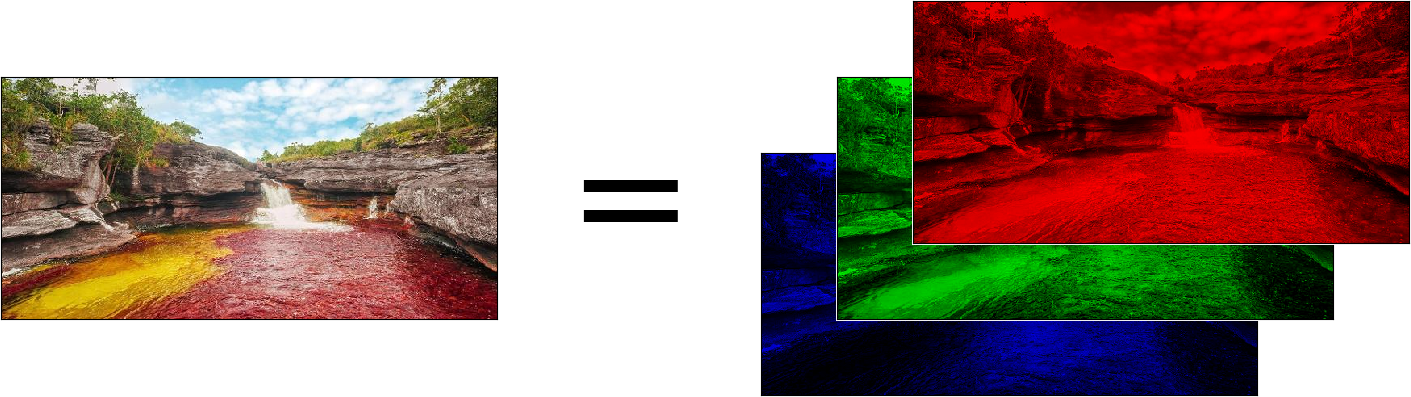
\includegraphics[width=\textwidth]{figs/canais-de-cor2.png}
        \caption{Fonte: Mario Carvajal}
    \end{figure}
\end{frame}

\begin{frame}{Decomposi\c{c}\~ao SVD}
    Dada $A_{m \times n}$, existem matrizes $U_{m \times m}$, $D_{m \times n}$
    e $V_{n \times n}$ tais que
    \[A = UDV^T\]

    \pause

    \begin{figure}
        \centering
        
\includegraphics[width=0.8\textwidth]{figs/svd1.pdf}
    \end{figure}
%    Por exemplo,
%    \begin{eqnarray}
%        \left[\begin{array}{cc}
%            a_{11} & a_{12} \\
%            a_{21} & a_{22}
%        \end{array}\right]
%        & = &
%        \left[\begin{array}{cc}
%            u_{11} & u_{12} \\
%            u_{21} & u_{22}
%        \end{array}\right]
%        \left[\begin{array}{cc}
%            d_{11} & 0 \\
%            0 & d_{22}
%        \end{array}\right]
%        \left[\begin{array}{cc}
%            v_{11} & v_{21} \\
%            v_{12} & v_{22}
%        \end{array}\right] \nonumber \\
%        & = &
%        d_{11}
%        \left[\begin{array}{c}
%            u_{11} \\
%            u_{21}
%        \end{array}\right]
%        \left[\begin{array}{cc}
%            v_{11} & v_{21}
%        \end{array}\right]
%        +
%        d_{22}
%        \left[\begin{array}{c}
%            u_{12} \\
%            u_{22}
%        \end{array}\right]
%        \left[\begin{array}{cc}
%            v_{12} & v_{22}
%        \end{array}\right] \nonumber 
%    \end{eqnarray}
\end{frame}

\begin{frame}{Decomposi\c{c}\~ao SVD}
    Dada $A_{m \times n}$, existem matrizes $U_{m \times m}$, $D_{m \times n}$
    e $V_{n \times n}$ tais que
    \[A = UDV^T\]


    \begin{figure}
        \centering
        
\includegraphics[width=0.8\textwidth]{figs/svd2.pdf}
    \end{figure}
\end{frame}

\begin{frame}{Decomposi\c{c}\~ao SVD}
    \begin{figure}
        \centering
        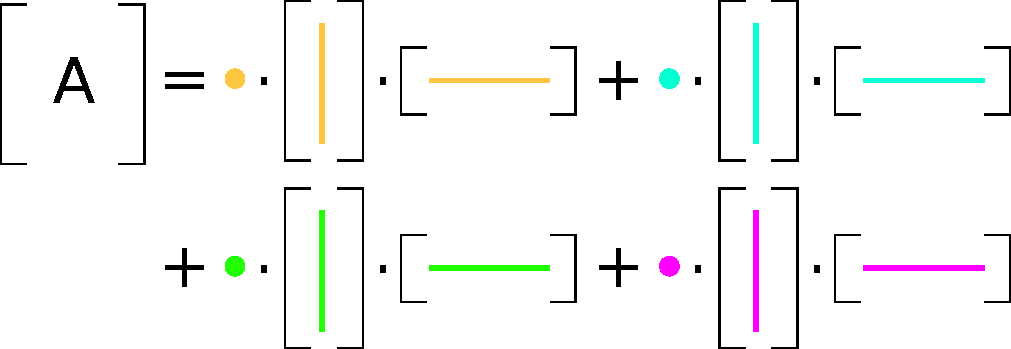
\includegraphics[width=0.8\textwidth]{figs/svd3.pdf}
    \end{figure}
\end{frame}

\begin{frame}{Decomposi\c{c}\~ao SVD}
    \begin{figure}
        \centering
        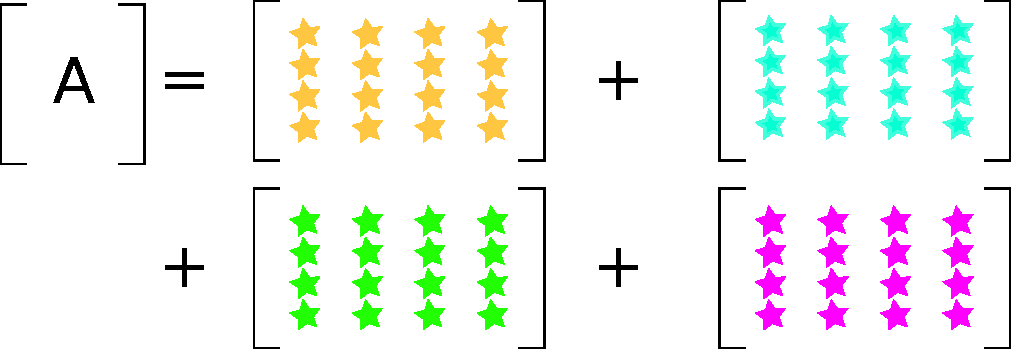
\includegraphics[width=0.8\textwidth]{figs/svd4.pdf}
    \end{figure}
\end{frame}

\begin{frame}{Compress\~ao de imagem}{Imagem original}
    \begin{figure}
        \centering
        \includegraphics[width=0.75\textwidth]{figs/navio-original.png}
        \caption{Tamanho: $2448 \times 3264$}
    \end{figure}
    \pause
    \begin{center}
        N\'umeros reais: $2448\times3264\times3=23.970.816$
    \end{center}
\end{frame}

\begin{frame}{Compress\~ao de imagem}{
    $A \approx d_{1,1}\cdot u(:,1)\cdot v(1,:)$}
    \pause
    \begin{figure}
        \centering
        \includegraphics[width=0.75\textwidth]{implementacao/out/nova1.png}
        \caption{Apenas 1 parcela}
    \end{figure}
    \begin{center}
        N\'umeros reais: $(1 + 2448 + 3264) \times 3 = 17.139\ (0,07\%)$
    \end{center}
\end{frame}

\begin{frame}{Compress\~ao de imagem}{
    $A \approx d_{1,1}\cdot u(:,1)\cdot v(1,:) + d_{2,2}\cdot
    u(:,2)\cdot v(2,:) +\cdots+ d_{50,50}\cdot u(:,50)\cdot v(50,:)$}
    \pause
    \begin{figure}
        \centering
        \includegraphics[width=0.75\textwidth]{implementacao/out/nova50.png}
        \caption{Com 50 parcelas}
    \end{figure}
    \begin{center}
        N\'umeros reais: $(1 + 2448 + 3264)\times 50 \times 3 = 856.950\ (3,5\%)$
    \end{center}
\end{frame}

\begin{frame}{Compress\~ao de imagem}{
    $A \approx d_{1,1}\cdot u(:,1)\cdot v(1,:) + d_{2,2}\cdot
    u(:,2)\cdot v(2,:) +\cdots+ d_{100,100}\cdot u(:,100)\cdot v(100,:)$}
    \begin{figure}
        \centering
        \includegraphics[width=0.75\textwidth]{implementacao/out/nova100.png}
        \caption{Com 100 parcelas}
    \end{figure}
    \begin{center}
        N\'umeros reais: $(1 + 2448 + 3264)\times 100 \times 3 = 1.713.900\ (7,1\%)$
    \end{center}
\end{frame}

\begin{frame}{Compress\~ao de imagem}{
    $A \approx d_{1,1}\cdot u(:,1)\cdot v(1,:) + d_{2,2}\cdot
    u(:,2)\cdot v(2,:) +\cdots+ d_{200,200}\cdot u(:,200)\cdot v(200,:)$}
    \begin{figure}
        \centering
        \includegraphics[width=0.75\textwidth]{implementacao/out/nova200.png}
        \caption{Com 200 parcelas}
    \end{figure}
    \begin{center}
        N\'umeros reais: $(1 + 2448 + 3264)\times 200 \times 3 = 3.427.800\ (14,3\%)$
    \end{center}
\end{frame}

%\begin{frame}{Vantagens}
%    \begin{itemize}
%        \item armazenamento
%        \item banda para transmiss\~ao (streaming)
%    \end{itemize}
%\end{frame}
%
%\begin{frame}{Desvantagens}
%    \begin{itemize}
%        \item processamento para reconstru\c{c}\~ao
%    \end{itemize}
%\end{frame}

\begin{frame}{Perguntas}
    \begin{figure}
        \centering
        
\includegraphics[height=\textheight]{figs/perguntas.png}
    \end{figure}
\end{frame}

\begin{frame}
    \begin{figure}
        \centering
        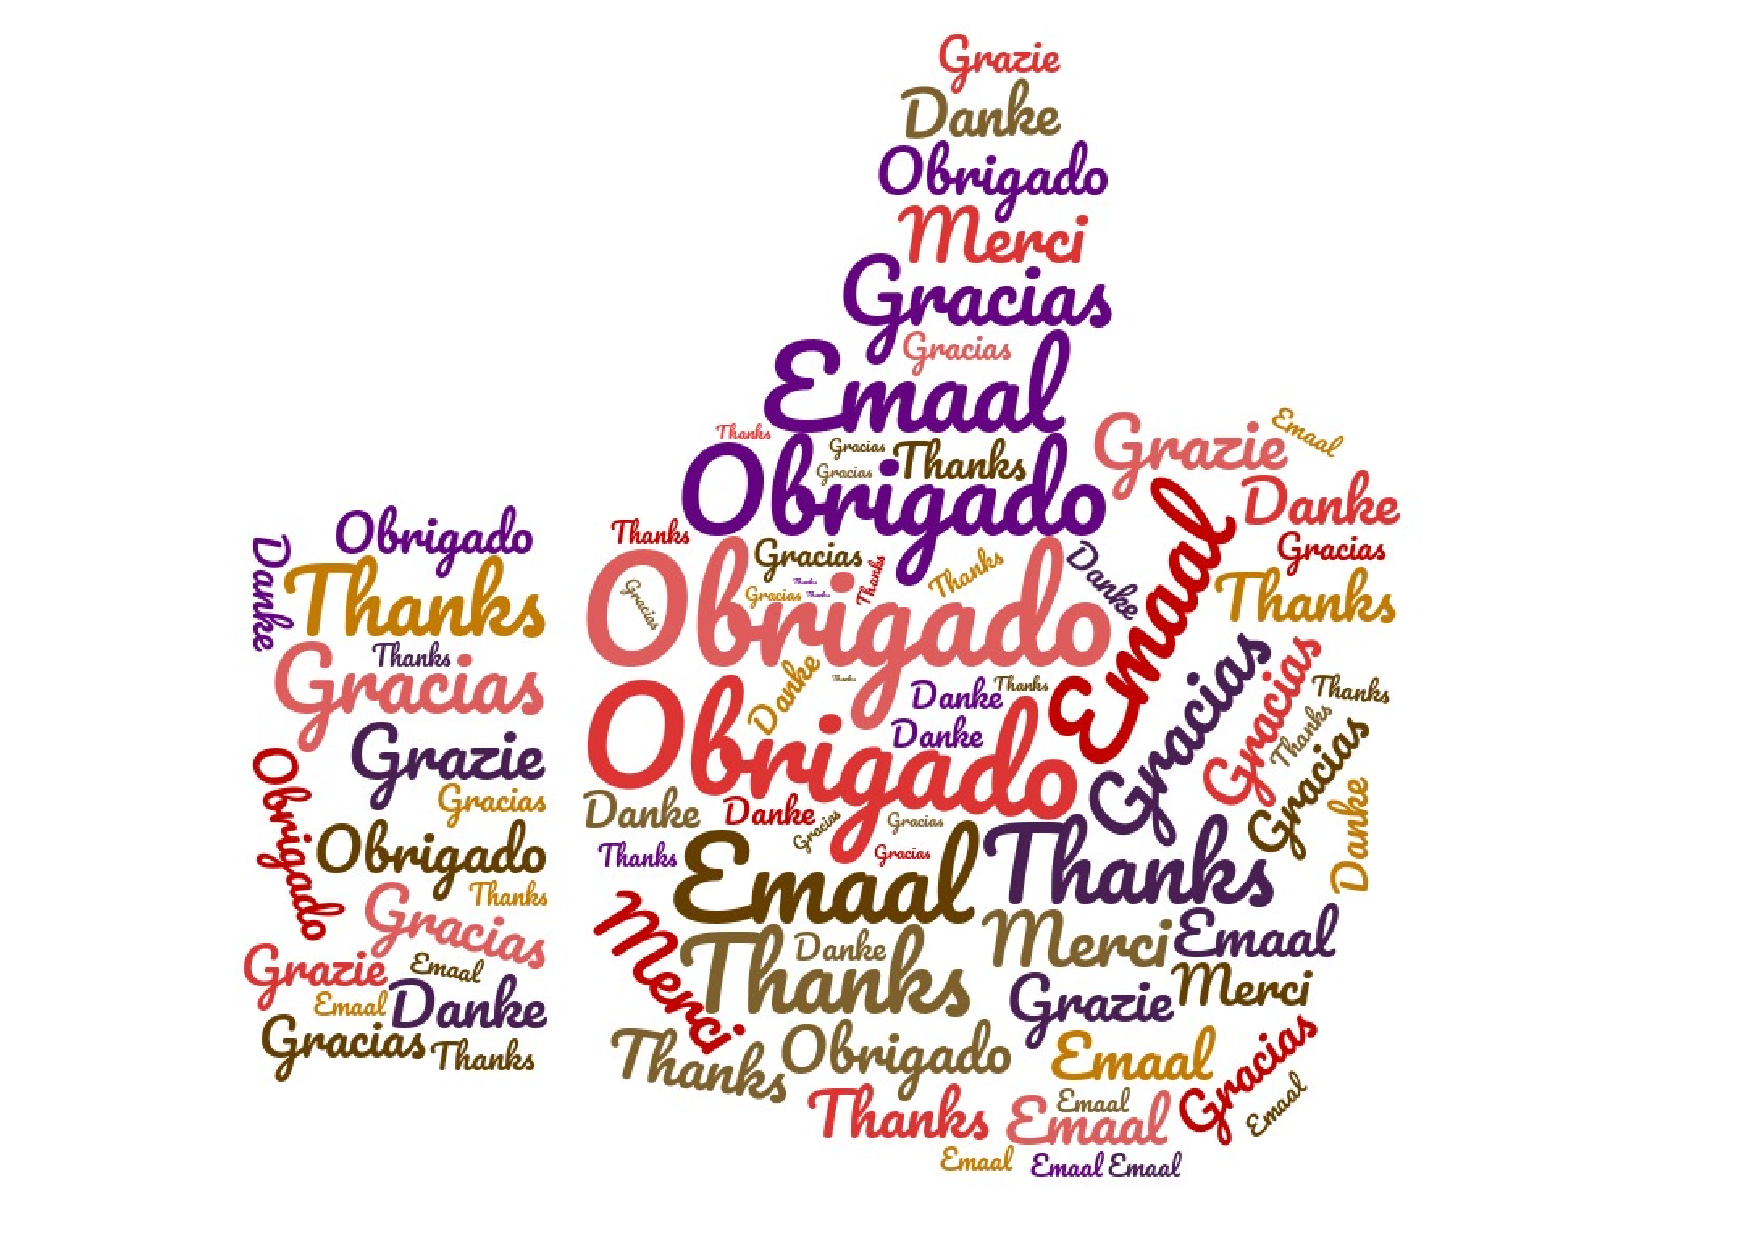
\includegraphics[width=0.9\textwidth]{figs/obrigado.pdf}
    \end{figure}
\end{frame}

\end{document}
